

\tikzset{every picture/.style={line width=0.75pt}} %set default line width to 0.75pt        

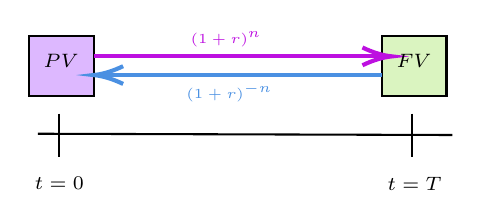
\begin{tikzpicture}[x=0.75pt,y=0.75pt,yscale=-1,xscale=1]
%uncomment if require: \path (0,300); %set diagram left start at 0, and has height of 300

%Straight Lines [id:da001] - Main timeline
\draw    (198,173) -- (397.68,173.61) ;
%Straight Lines [id:da002] - Vertical tick at t=0
\draw    (208.2,163.27) -- (208.2,184.27) ;
%Straight Lines [id:da003] - Vertical tick at t=n
\draw    (378.2,163.27) -- (378.2,184.27) ;

%Shape: Rectangle [id:dp001] - PV at t=0
\draw  [fill={rgb, 255:red, 144; green, 19; blue, 254 }  ,fill opacity=0.3 ] (193.53,125.73) -- (224.81,125.73) -- (224.81,154.73) -- (193.53,154.73) -- cycle ;
%Shape: Rectangle [id:dp002] - FV at t=n
\draw  [fill={rgb, 255:red, 184; green, 233; blue, 134 }  ,fill opacity=0.52 ] (363.53,125.73) -- (394.81,125.73) -- (394.81,154.73) -- (363.53,154.73) -- cycle ;

%Straight Lines [id:da004] - Forward arrow (capitalization)
\draw [color={rgb, 255:red, 189; green, 16; blue, 224 }  ,draw opacity=1 ][line width=1.5]    (224.81,135.73) -- (365.53,135.73) ;
\draw [shift={(368.53,135.73)}, rotate = 180] [color={rgb, 255:red, 189; green, 16; blue, 224 }  ,draw opacity=1 ][line width=1.5]    (14.21,-4.28) .. controls (9.04,-1.82) and (4.3,-0.39) .. (0,0) .. controls (4.3,0.39) and (9.04,1.82) .. (14.21,4.28)   ;

%Straight Lines [id:da005] - Backward arrow (discounting)
\draw [color={rgb, 255:red, 74; green, 144; blue, 226 }  ,draw opacity=1 ][line width=1.5]    (363.53,144.73) -- (227.81,144.73) ;
\draw [shift={(224.81,144.73)}, rotate = 360] [color={rgb, 255:red, 74; green, 144; blue, 226 }  ,draw opacity=1 ][line width=1.5]    (14.21,-4.28) .. controls (9.04,-1.82) and (4.3,-0.39) .. (0,0) .. controls (4.3,0.39) and (9.04,1.82) .. (14.21,4.28)   ;

% Text Node
\draw (195,192.4) node [anchor=north west][inner sep=0.75pt]  [font=\scriptsize]  {$t=0$};
% Text Node
\draw (365,192.4) node [anchor=north west][inner sep=0.75pt]  [font=\scriptsize]  {$t=T$};
% Text Node
\draw (209.17,137.83) node [anchor=center][inner sep=0.75pt]  [font=\scriptsize]  {$PV$};
% Text Node
\draw (379.17,137.83) node [anchor=center][inner sep=0.75pt]  [font=\scriptsize]  {$FV$};
% Text Node - Capitalization label
\draw (270,122.4) node [anchor=north west][inner sep=0.75pt]  [font=\tiny,color={rgb, 255:red, 189; green, 16; blue, 224 }]  {$(1+r)^{n}$};
% Text Node - Discounting label
\draw (268,147.4) node [anchor=north west][inner sep=0.75pt]  [font=\tiny,color={rgb, 255:red, 74; green, 144; blue, 226 }]  {$(1+r)^{-n}$};


\end{tikzpicture}
